\section{Experimental Results}
\ifCLASSOPTIONonecolumn\begin{figure*}[t]
\centering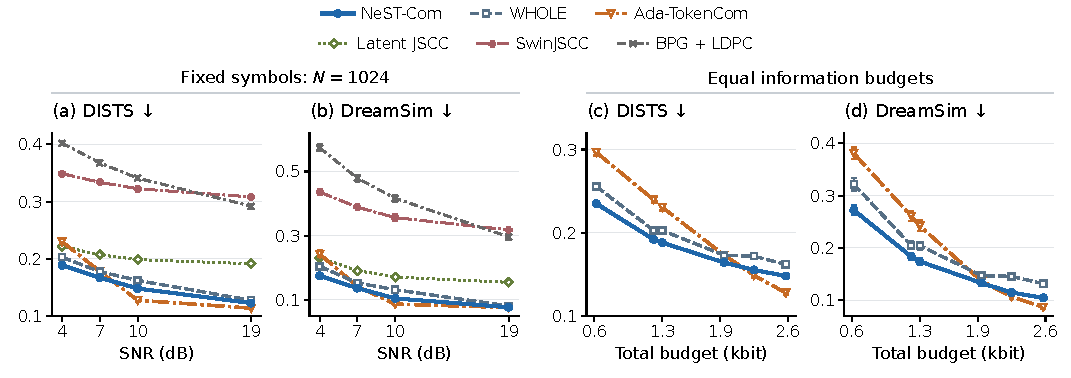
\includegraphics[width=\linewidth]{figure2.pdf}
\caption{Source-referenced reconstruction on common500. (a,b) Seven systems at $N=1024$, averaging three channel outcomes per source including failures. (c,d) Error-free equal-information budgets, including 57 shared overhead bits and Ada's additional 10-bit class; WHOLE/NeST share ceiling $(10,0)$. Points and bars are equal-source means and pointwise 95\% source-bootstrap intervals. Ada is the predicted-class fixed-frame adaptation. Lower values are favorable.}
\label{fig:performance}\end{figure*}
\fi
\subsection{Setup and Calibration Protocol}
We test 500 ImageNet validation images~\cite{imagenet}, disjoint from 1000 calibration images, at $256\times256$: $N=1024$ at 4/7/10/19 dB and $N=512$ at 4/10/19 dB. We average three realizations per image, including gray failures, then compute equal-source means and direct paired 95\% intervals using 10\,000 source resamples. Controls use a fixed 100-image subset. Calibrated token systems and matched controls share noise; external systems retain their original noise.

Latent JSCC maps tokenizer latents to symbols and shares $\Dc$ (MSE, LPIPS and latent-consistency losses, 100k updates). SwinJSCC~\cite{swinjscc} uses RGB MSE (200k updates, calibration-MSE selection). Both train on 20\,000 images at $N=1024$. BPG~\cite{bpg} uses LDPC/QAM. Ada-TokenCom~\cite{adatokencom} is a predicted-class, fixed-frame adaptation: LlamaGen-L/VQ16, prefix arithmetic coding, CFG=4, $T=1$, top-$k=2000$, top-$p=1$, and a paid 10-bit ConvNeXt class. Long-term control and ARQ are excluded.

DISTS~\cite{dists}, DreamSim~\cite{dreamsim}, PSNR, LPIPS-Alex~\cite{lpips} and CLIP-I~\cite{clip} use native float RGB with fixed preprocessing. Timing uses 32 images, two warmups, three measurements, batch one, one RTX PRO 6000 and two physical CPU cores. We separately measure GPU-synchronized TX (RGB-to-symbols) and RX (symbols-to-RGB) processing times. They include coding, link processing and generation, excluding loading, I/O and scoring; total processing time is their sum. Supplementary Sections~S2--S8 give complete results, controls, examples, timing and transfer details, including ARPC's specified digital-link adaptation.

Policies are calibrated once and then frozen. At $N=1024$, WHOLE, NeST and Ada share 12 MCSs combining QPSK, 16-QAM or 64-QAM with code rates $1/2$, $2/3$, $3/4$ or $5/6$. WHOLE has seven ceilings, NeST uses 25 Quarter ceilings with Token fallback, and Ada allows prefixes through 256 tokens. All 396 candidates are screened on 100 calibration images with one noise realization. For each method and SNR, the top three candidates and a preset QPSK rate-$1/2$ anchor advance to 1000 calibration images with three realizations each. The highest equal-source mean DINOv2 cosine similarity~\cite{dinov2}, including gray failures, determines the policy. The $N=512$ policies are calibrated separately (Table~\ref{tab:policies}).

\begin{table}[t]
\caption{Within-scale transmission. (A) Shared-model NeST--WHOLE differences. (B) Matched endpoint granularity. (C) Ordered receiver interventions. Brackets are source-paired 95\% intervals; sample sizes are specified for each block.}
\label{tab:internal}\centering\footnotesize
\setlength{\tabcolsep}{2.1pt}\renewcommand{\arraystretch}{1.05}
\begin{tabular}{@{}lccc@{}}\toprule
\multicolumn{4}{l}{\textit{A. 500 sources, $N=1024$, uniformly calibrated policies}}\\
SNR & Util. W$\to$N (\%) & $\Delta$DISTS & $\Delta$DreamSim\\
\midrule
4 & 73.81$\to$99.56 & \shortstack{-0.0142\\{}[-0.0155, -0.0127]} & \shortstack{-0.0297\\{}[-0.0330, -0.0264]}\\[2pt]
7 & 83.19$\to$99.71 & \shortstack{-0.0103\\{}[-0.0139, -0.0068]} & \shortstack{-0.0159\\{}[-0.0207, -0.0112]}\\[2pt]
10 & 77.70$\to$99.79 & \shortstack{-0.0141\\{}[-0.0153, -0.0128]} & \shortstack{-0.0270\\{}[-0.0299, -0.0241]}\\[2pt]
19 & 85.24$\to$99.83 & \shortstack{-0.0048\\{}[-0.0053, -0.0043]} & \shortstack{-0.0043\\{}[-0.0051, -0.0036]}\\[2pt]
\bottomrule\end{tabular}
\par\smallskip
\begin{tabular}{@{}lrrrr@{}}\toprule
\multicolumn{5}{l}{\textit{B. 100 quality sources; 32 timing sources; ceiling $(8,126)$}}\\
Grid & Util. (\%) & DISTS & DreamSim & TX (ms)\\\midrule
Whole & 78.13 & 0.1650 & 0.1387 & 185.2\\
Quarter & 95.19 & 0.1535 & 0.1143 & 215.8\\
Eighth & 97.44 & 0.1516 & 0.1137 & 217.8\\
Token & 99.85 & 0.1505 & 0.1115 & 248.4\\
\bottomrule\end{tabular}
\par\smallskip
\begin{tabular}{@{}lccc@{}}\toprule
\multicolumn{4}{l}{\textit{C. 100 sources, 10 dB, same received prefixes}}\\
Intervention & $\Delta$PSNR (dB) & $\Delta$DISTS & $\Delta$DreamSim\\
\midrule
B0--A0 & \shortstack{+0.287\\{}[0.240, 0.335]} & \shortstack{-0.0062\\{}[-0.0077, -0.0048]} & \shortstack{-0.0113\\{}[-0.0147, -0.0083]}\\[2pt]
C0--B0 & \shortstack{+0.537\\{}[0.404, 0.682]} & \shortstack{-0.0083\\{}[-0.0102, -0.0065]} & \shortstack{-0.0159\\{}[-0.0205, -0.0116]}\\[2pt]
\bottomrule\end{tabular}
\par\smallskip
\begin{minipage}{\columnwidth}\scriptsize
A0: prior completion without received boundary tokens. B0: A0 plus boundary residual correction. C0: B0 plus updated finer-scale conditioning.
\end{minipage}
\end{table}

\ifCLASSOPTIONonecolumn\else\begin{figure*}[t]
\centering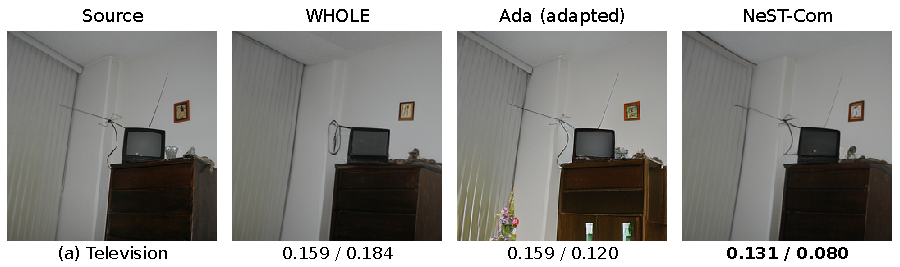
\includegraphics[width=6.0in]{figure3.pdf}
\caption{Selected reconstruction examples at $N=1024$ and 10 dB. Columns show source, WHOLE, SwinJSCC, the predicted-class fixed-frame Ada-TokenCom adaptation, and NeST-Com. Values are full-image DISTS$\downarrow$ / DreamSim$\downarrow$ for each method's first prescribed channel realization. Supplement~S6 gives source identities, selection details and additional examples.}
\label{fig:qualitative}\end{figure*}
\fi
\subsection{Within-Scale Fitting and Mechanism Attribution}
Table~\ref{tab:internal}(C) isolates the receiver's use of boundary tokens by holding the received NeST prefixes fixed. A0 predicts the boundary and finer maps from the complete coarse maps. B0 applies the received tokens to correct the boundary residual while retaining A0's finer-scale conditioning. C0 also uses the corrected boundary map to condition the finer scales. At 10 dB, B0 improves PSNR by 0.287 dB over A0, and C0 adds 0.537 dB over B0. The paired PSNR, DISTS and DreamSim intervals favor both steps.

In the 500-image comparison, NeST and WHOLE share the model, coder and receiver and use separately calibrated policies. At $N=1024$ and 10 dB, source-bit capacity utilization rises from 77.70\% to 99.79\%, mean DISTS falls from 0.1621 to 0.1481, and mean DreamSim falls from 0.1317 to 0.1048. Table~\ref{tab:internal}(A) reports the paired NeST--WHOLE differences computed before rounding, $-0.0141$ for DISTS and $-0.0270$ for DreamSim. At the same operating point, mean PSNR increases from 19.31 dB for WHOLE to 20.19 dB for NeST, a gain of 0.88 dB (Table~\ref{tab:external}). All five paired metrics favor NeST at all seven budget/SNR points (Supplement~S2).

Table~\ref{tab:internal}(B) isolates granularity on a separate 100-image quality subset by fixing the model, 16-QAM rate 2/3, ceiling $(8,126)$, fitting rule and noise. Eighth retains approximately 92\% of the Whole-to-Token gain in PSNR, DISTS and DreamSim. Token raises utilization from 97.44\% to 99.85\%, adding $0.066\,[0.034,0.101]$ dB PSNR, with DISTS/DreamSim differences $-0.0011\,[-0.0020,-0.0002]$/$-0.0022\,[-0.0042,-0.0001]$, at 30.7 ms (14.1\%) additional TX cost. Eighth offers lower cost; Token prioritizes fuller capacity use and the additional measured quality gain.

\subsection{System-Level Comparison}
\ifCLASSOPTIONonecolumn\begin{figure*}[t]
\centering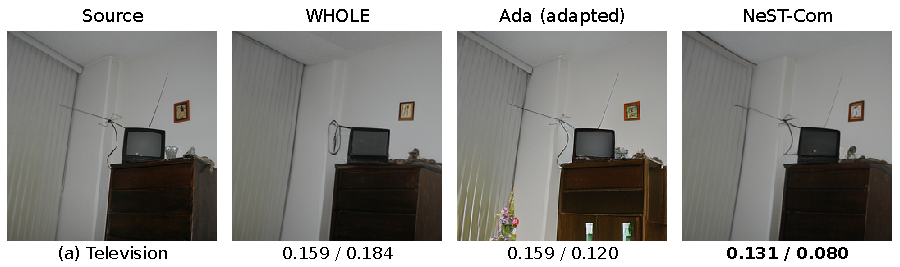
\includegraphics[width=6.0in]{figure3.pdf}
\caption{Selected reconstruction examples at $N=1024$ and 10 dB. Columns show source, WHOLE, SwinJSCC, the predicted-class fixed-frame Ada-TokenCom adaptation, and NeST-Com. Values are full-image DISTS$\downarrow$ / DreamSim$\downarrow$ for each method's first prescribed channel realization. Supplement~S6 gives source identities, selection details and additional examples.}
\label{fig:qualitative}\end{figure*}
\fi
\begin{table}[t]
\caption{Auxiliary quality on 500 test images at $N=1024$, 10 dB. Means include three realizations per source and gray failures.}
\label{tab:external}\centering\footnotesize\setlength{\tabcolsep}{5pt}
\begin{tabular}{@{}lrrr@{}}\toprule
Method & PSNR (dB)$\uparrow$ & LPIPS$\downarrow$ & CLIP-I$\uparrow$\\\midrule
WHOLE & 19.31 & 0.199 & 0.858\\
NeST-Com & 20.19 & 0.166 & 0.877\\
Ada-TokenCom & 19.56 & 0.167 & 0.884\\
Latent JSCC & 20.80 & 0.173 & 0.789\\
SwinJSCC & 23.03 & 0.469 & 0.669\\
BPG + LDPC & 22.54 & 0.589 & 0.635\\
\bottomrule\end{tabular}\end{table}

Fig.~\ref{fig:performance}(a,b) compares six methods at equal symbol budgets. NeST has lower DISTS and DreamSim than SwinJSCC, Latent JSCC and BPG at all four $N=1024$ SNRs (24 paired intervals excluding zero). SwinJSCC and BPG have higher PSNR.

Against Ada, NeST improves both distances at 4 dB and DISTS at 7 dB. Ada has lower distances at 10 dB and lower DISTS at 19 dB. NeST has higher PSNR at all four SNRs. At 7 dB, WHOLE, NeST and Ada reject 11, 7 and 10 of 1500 receptions, respectively. NeST rejects one frame at 4 dB. All other token-system points have zero rejections, and no valid NULL frames occur. Table~\ref{tab:external} gives auxiliary metrics at 10 dB.

Fig.~\ref{fig:performance}(c,d) compares the schemes at six equal, error-free information budgets (620--2577 bits), including 57 shared protocol bits and Ada's additional 10-bit class. NeST improves all five metrics over WHOLE. Against Ada, DISTS favors NeST at the four smallest budgets and DreamSim at the first three. Ada has lower values on both metrics at 2248 and 2577 bits.

\subsection{Reduced Budget, Transfer and Threshold Behavior}
\begin{table}[t]
\caption{Reduced-budget reconstruction on 500 sources at $N=512$. Means include all failures; PSNR differences use direct source-paired 95\% intervals. All five metrics and paired comparisons are in Supplement~S2.}
\label{tab:reduced}\centering\footnotesize\setlength{\tabcolsep}{3pt}
\begin{tabular}{@{}lrrr@{}}\toprule
SNR / method & PSNR$\uparrow$ & DISTS$\downarrow$ & DreamSim$\downarrow$\\
\midrule
4 / WHOLE & 15.11 & 0.2580 & 0.3247\\
4 / NeST-Com & 15.61 & 0.2363 & 0.2740\\
4 / Ada-TokenCom & 11.32 & 0.2996 & 0.3847\\
\multicolumn{4}{l}{NeST--WHOLE $\Delta$PSNR: +0.504 [0.440, 0.573] dB}\\
\midrule
10 / WHOLE & 16.82 & 0.2030 & 0.2049\\
10 / NeST-Com & 17.41 & 0.1922 & 0.1837\\
10 / Ada-TokenCom & 13.16 & 0.2367 & 0.2582\\
\multicolumn{4}{l}{NeST--WHOLE $\Delta$PSNR: +0.592 [0.544, 0.643] dB}\\
\midrule
19 / WHOLE & 18.64 & 0.1718 & 0.1458\\
19 / NeST-Com & 19.63 & 0.1554 & 0.1150\\
19 / Ada-TokenCom & 17.69 & 0.1496 & 0.1078\\
\multicolumn{4}{l}{NeST--WHOLE $\Delta$PSNR: +0.994 [0.940, 1.048] dB}\\
\bottomrule\end{tabular}\end{table}

\begin{table}[t]
\caption{Frozen policies: MCS entries are (bits/symbol, code rate); $e$ is the target ceiling, with feasible fallback. Ada's ceiling is 256 tokens. Budgets are calibrated independently.}
\label{tab:policies}\centering\footnotesize\setlength{\tabcolsep}{2.5pt}
\begin{tabular}{@{}lccccc@{}}\toprule
$N$/SNR & $a_{\rm W}$ & $e_{\rm W}$ & $a_{\rm N}$ & $e_{\rm N}$ & $a_{\rm Ada}$\\\midrule
1024/4 & $2,2/3$ & $(7,0)$ & $2,2/3$ & $(7,25)$ & $2,2/3$\\
1024/7 & $4,1/2$ & $(8,0)$ & $4,1/2$ & $(8,0)$ & $4,1/2$\\
1024/10 & $4,2/3$ & $(9,0)$ & $4,2/3$ & $(8,126)$ & $4,2/3$\\
1024/19 & $6,5/6$ & $(10,0)$ & $6,5/6$ & $(10,0)$ & $4,5/6$\\
512/4 & $2,2/3$ & $(6,0)$ & $2,2/3$ & $(5,27)$ & $2,2/3$\\
512/10 & $4,2/3$ & $(7,0)$ & $4,2/3$ & $(7,0)$ & $4,2/3$\\
512/19 & $6,5/6$ & $(8,0)$ & $6,5/6$ & $(8,84)$ & $6,5/6$\\
\bottomrule\end{tabular}\end{table}

The $N=512$, 10-dB granularity control fixes 100 images, three shared noise realizations, 16-QAM at rate $2/3$, ceiling $(7,0)$, model and receiver. Eighth retains 87\% of the Whole-to-Token PSNR gain. Token further improves PSNR, LPIPS and DreamSim, with DISTS and CLIP-I intervals crossing zero.

On the 500 test images at $N=512$, all five paired intervals favor NeST over WHOLE at all three SNRs. PSNR gains range from 0.50 to 0.99 dB (Table~\ref{tab:reduced}). At 10 dB both methods use ceiling $(7,0)$ and 16-QAM at rate $2/3$, and utilization rises from 79.30\% to 99.54\%.

We evaluate 24 Kodak center crops using ImageNet-calibrated policies, with 64-QAM at code rate $5/6$ for Ada at 19 dB. NeST improves PSNR, DISTS and DreamSim over WHOLE at all three SNRs, and all 864 receptions succeed.

\subsection{Operation Near the Channel Threshold}
With the earlier 10-dB policies fixed, 100 sources and 20 noise realizations per point yield 30\,000 receptions over 8--10 dB. All three methods reject every frame at 8 dB. WHOLE/NeST/Ada rejection rates are 15.75/14.95/13.50\% at 9 dB, 0.10--0.20\% at 9.5 dB and zero observed at 10 dB. Gray failures enter overall quality (S5). Reconstruction gains require a sufficiently reliable digital link.


Fig.~\ref{fig:qualitative} illustrates NeST preserving truck markings and foreground contours. These selected cases favor NeST in DISTS and DreamSim and SwinJSCC in PSNR.

We measure processing time for each token system at $N=1024$ and 10 dB using 16-QAM at code rate $2/3$ and the corresponding source-prefix ceiling in Table~\ref{tab:policies}. TX and RX take 248.44 and 403.99 ms for NeST, respectively, and 215.29 and 366.42 ms for WHOLE. Total processing time is 652.43 ms for NeST and 39.17 ms for SwinJSCC. The 3.064 s measured for compiled Ada is paired with its own 32-image quality evaluation. The main Ada quality results use the original implementation.
